
% slides for Ph.D students day

\documentclass{beamer} % oral talk
%\documentclass[trans]{beamer}  % paper version
\mode<presentation> {
  %\usetheme{Darmstadt}
  \usetheme{Madrid}
  \usecolortheme{crane}
  %\usetheme{Goettingen}
  %\usecolortheme{wolverine}
  \setbeamercovered{transparent}
  %\useoutertheme{sidebar}
}
\usepackage{graphicx}
\usepackage{xspace}
\usepackage[dvips]{epsfig}
\usepackage{xmpmulti}
\usepackage{color}
\usepackage{colortbl}
\usepackage{setspace}
\usepackage{array}
\usepackage{latexsym}
\usepackage{comment}
\usepackage{amssymb,amsmath,amsthm}

\usepackage {bussproofs}
\bottomAlignProof

\usepackage{dednatcol}
\usepackage{alltt}
\usepackage[latin1]{inputenc}
\usepackage{times}
\usepackage[T1]{fontenc}
\usepackage[english]{babel}

\definecolor{Blue}{rgb}{0.1,0.1,0.8}

\newcommand{\keywd}[1]{\textbf{#1}}

\setbeamercovered{dynamic}
\setbeamertemplate{theorems}[numbered]

\newcommand{\hs}{\hspace{1cm}}
\newcommand{\vs}{\vspace{1cm}}
\newcommand{\vsfive}{\vspace{5mm}}
\newcommand{\hsfive}{\hspace{5cm}}

\newcommand{\mboxfill}{\mbox{ }\hfill}

% Variables logiques

\newcommand{\rv}{\bleu {rv}\xspace}
\newcommand{\re}{\bleu {re}\xspace}
\newcommand{\rg}{\bleu {rg}\xspace}
\newcommand{\rd}{\bleu {rd}\xspace}

\newcommand{\pv}[1]{{\bleu {\textsf{I}}(\marron{#1})}}
\newcommand{\pe}[1]{{\bleu {\textsf{W}}(\marron{#1})}}
\newcommand{\pg}[1]{{\bleu {\textsf{S}}(\marron{#1})}}
\newcommand{\pd}[1]{{\bleu {\textsf{D}}(\marron{#1})}}

\newcommand{\vv}[1]{{\bleu {I}(\ensuremath{\vav{#1}})}}
\newcommand{\ve}[1]{{\bleu {W}(\ensuremath{\vav{#1}})}}
\newcommand{\vg}[1]{{\bleu {S}(\ensuremath{\vav{#1}})}}
\newcommand{\vd}[1]{{\bleu {D}(\ensuremath{\vav{#1}})}}

\newcommand{\mystrut}{\hbox to 0pt{\phantom{()}}}
%%%%%%%%%%%%%%%%%


\newtheorem{defn}{Definition}


%\newtheorem{theo}{Theorem}[section] % theorems are numbered by section
\newtheorem{theo}{Theorem} % theorems are numbered by section
\newtheorem{prop}[theo]{Proposition} % propositions are numbered as theorems
\newtheorem{lem}{Lemma} % lemmas are no longer numbered as theorems
\newtheorem{myfact}[theo]{Fact} % lemmas are numbered as theorems
\newtheorem{de}[theo]{Definition} % 

% \newcommand{\egdef}%
%    {\ensuremath{~\:\mathrel{\raisebox{-.7ex}%
%    {$\stackrel{\rm def}{=\mkern-8mu=}$}}\:~}}

\renewcommand{\impl}{\ensuremath{\Rightarrow}}


% \definecolor{marron}{rgb}{0.6, 0.2, 0}
% \definecolor{mygreen}{rgb}{0.0,0.5,0.0}
% \definecolor{brique}{rgb}{0.75, 0.05, 0}
% \definecolor{violet}{rgb}{.75, 0, .75}

% \definecolor{lightblue}{rgb}{0.75,0.85,1}
% \definecolor{lightred}{rgb}{1,0.8,0.8}
% \definecolor{lightgreen}{rgb}{0.6,1,0.6}
% \definecolor{semilightgreen}{rgb}{0.5,1,0.5}
% \definecolor{lightyellow}{rgb}{1.0,1.0,0.5}
% \definecolor{lightorange}{rgb}{1.0, 0.87, 0.01}

% \newcommand{\marron}[1]{\textcolor{marron}{#1}}
% \newcommand{\brun}[1]{\textcolor{brown}{#1}}
% \newcommand{\cvert}[1]{\textcolor{mygreen}{#1}}
% \newcommand{\bleu}[1]{\textcolor{blue}{#1}}
% \newcommand{\rouge}[1]{\textcolor{red}{#1}}
% \newcommand{\brique}[1]{\textcolor{brique}{#1}}
% \newcommand{\violet}[1]{\textcolor{violet}{#1}}

\newcommand{\cdat}{\violet}
\newcommand{\cloc}{\cvert}

% ----------------------------------------------------------------------
\newcommand{\loc}{\cloc{\textit{loc}}}
\newcommand{\lx}{\cloc{\textit{x}}}
\newcommand{\ly}{\cloc{\textit{y}}}

\newcommand{\edge}[2]{\ensuremath{\cloc{#1\!\mathbin{\rightarrow}\! #2}}}
\newcommand{\cdb}{\ensuremath{\mathcal{\cdat C}}}
\newcommand{\incdb}[1]{\ensuremath{#1\in\cdb}}
\newcommand{\nincdb}[1]{\ensuremath{#1\not\in\cdb}}
\newcommand{\cdbp}{\ensuremath{\cdat{\mathcal{C}'}}}
\newcommand{\incdbp}[1]{\ensuremath{#1\in\cdbp}}
\newcommand{\nincdbp}[1]{\ensuremath{#1\not\in\cdbp}}
\newcommand{\atloc}[1]{\cdat{\ensuremath{\left|\cloc{#1}\right|}}}
\newcommand{\inset}[2]{\ensuremath{#1\in#2}}
\newcommand{\inloc}[2]{\ensuremath{#1\in\atloc{#2}}}
\newcommand{\ninloc}[2]{\ensuremath{#1\not\in\atloc{#2}}}
\newcommand{\visloc}[2]{\ensuremath{#1\in\cdat{\overline{\atloc{#2}}}}}
\newcommand{\nvisloc}[2]{\ensuremath{#1\not\in\cdat{\overline{\atloc{#2}}}}}
\newcommand{\inedge}[3]{\inloc{#1}{\edge{#2}{#3}}}
\newcommand{\ninedge}[3]{\ninloc{#1}{\edge{#2}{#3}}}
\newcommand{\cnf}{\textit{\cdat{cnf}}}
\newcommand{\pre}{\cdat{\textit{pre}}}
\newcommand{\post}{\cdat{\textit{post}}}
\newcommand{\extconfpar}[2]{\cdat{\ensuremath{\langle #1, #2\rangle}}}
\newcommand{\extconf}{\extconfpar{\cnf}{\cdb}}
\newcommand{\extconfpre}{\extconfpar{\pre}{\cdb}}
\newcommand{\extconfpost}{\extconfpar{\post}{\cdbp}}
%\newcommand{\entails}{~\rhd~}
\newcommand{\entailstrans}{\:\xrightarrow{\:trans\:}\:} % general
\newcommand{\entailsp}{\:\xrightarrow{\:sr\:}\:} % pure synchronous round
\newcommand{\entailso}{\:\xrightarrow{\:or\:}\:} % oracle round
\newcommand{\entails}{\:\xrightarrow{\:sor\:}\:} % synchronous + oracle round
\newcommand{\roas}{\textsc{roas}}
\newcommand{\roasat}[2]{\ensuremath{\roas\,@\,\edge{#1}{#2}}}
\newcommand{\roasto}[1]{\ensuremath{\roas\,@\,\cloc{\overline{#1}}}}
\newcommand{\goodat}[2]{\ensuremath{good\,@\,\edge{#1}{#2}}}
\newcommand{\goodto}[1]{\ensuremath{good\,@\,\cloc{\overline{#1}}}}
\newcommand{\correctonSTat}[1]{\ensuremath{\mbox{correct-onST}\,@\,\cloc{#1}}}
\newcommand{\wcorrectonSTat}[1]{\ensuremath{\mbox{weak-correct-onST}\,@\,\cloc{#1}}}
\newcommand{\completeonSTat}[1]{\ensuremath{\mbox{complete-onST}\,@\,\cloc{#1}}}
\newcommand{\readyat}[1]{\ensuremath{\mbox{ready}\,@\,\cloc{#1}}}
\newcommand{\correctSTat}[1]{\ensuremath{\mbox{correct-ST}\,@\,\cloc{#1}}}
\newcommand{\completeSTat}[1]{\ensuremath{\mbox{complete-ST}\,@\,\cloc{#1}}}
\newcommand{\invarat}[1]{\ensuremath{\mbox{invar}\,@\,\cloc{#1}}}


\title{An impredicative encoding of inversion}
%\subtitle{No subtitle}
\author[X. Shi] % (optional, nur bei vielen Autoren)
{\underline{Xiaomu Shi}\\Jean-Fran\c{c}ois Monin}

\institute[LIAMA \& Univ Grenoble]

\date[Beijing, March 02, 2012]

\begin{document}

\frame{\titlepage

\vfill

}

\section<presentation>*{Outline}

\begin{frame}
  \frametitle{Outline}
  \tableofcontents%[part=1,pausesections]
\end{frame}


%\AtBeginSubsection[] {
\AtBeginSection[] {
  \begin{frame}<beamer>
    \frametitle{Outline}
    \tableofcontents[current,subsection]
  \end{frame}
}


%%%%%%%%%%%%%%%%%%%%%%%%%%%%%%%%%%%%%%%%%%%%%%%%%%%
%%%%%%%%%%%%%%%%%%%%%%%%%%%%%%%%%%%%%%%%%%%%%%%%%%%
\section{Recall}
\begin{frame}[fragile]
\frametitle{SimSoC-Cert}
\hfil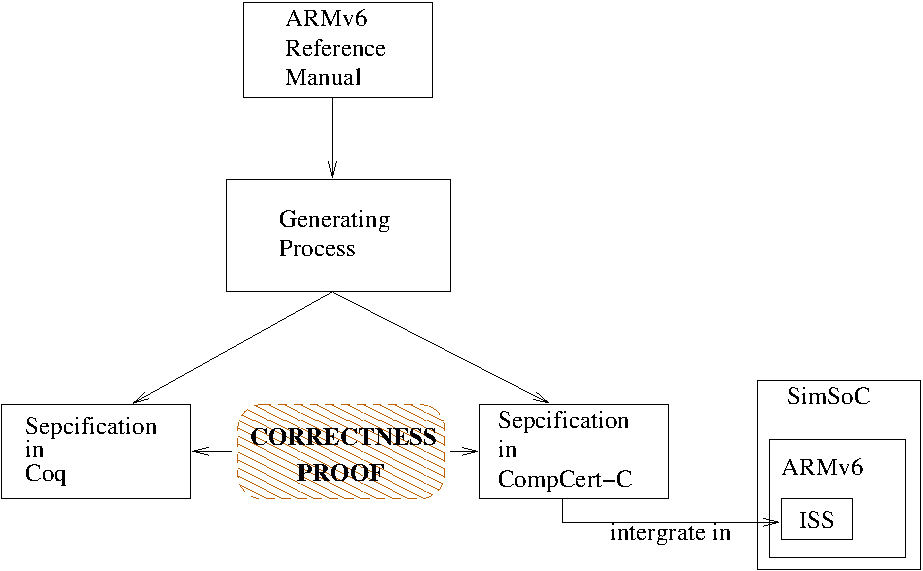
\includegraphics[width=.8\linewidth]{thumbnail.pdf}
\end{frame}

\begin{frame}[fragile]
\frametitle{Main theorem of SimSoC-Cert}
\hfil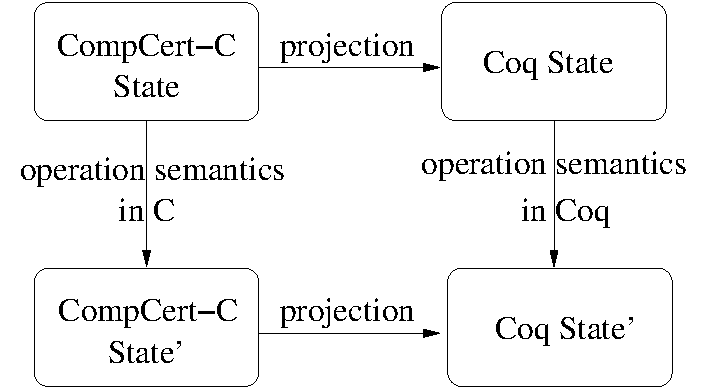
\includegraphics[width=.8\linewidth]{theorem.pdf}
%Make the pic colorful
\end{frame}
%%%%%%%%%%%%%%%%%%%%%%%%%%%%%%%%%%%%%%%%%%%%%%%%%%%

%%%%%%%%%%%%%%%%%%%%%%%%%%%%%%%%%%%%%%%%%%%%%%%%%%%
\section{Inversion issues in our project}

%%%%%%%%%%%%%%%%%%%%%%%%%%%%%%%%%%%%%%%%%%%%%%%%%%%

\subsection{Big inductive type from CompCert}
\begin{frame}[fragile]
\frametitle{Big inductive type from CompCert}
\begin{block}{eval\_expr}
In CompCert, the evaluation of an expression is defined as follows. \\
15 constructors. One of the most used types in our proofs.
\end{block}
\small
\begin{alltt}
\tiny
Inductive eval\_expression: env -> mem -> expr -> trace -> mem -> val -> Prop :=
  | eval\_expression\_intro: forall e m a t m' a' v,
      eval\_expr e m RV a t m' a' -> eval\_simple\_rvalue ge e m' a' v ->
      eval\_expression e m a t m' v
with \brique{eval\_expr}: env -> mem -> kind -> expr -> trace -> mem -> expr -> Prop :=
  | eval\_val: forall e m v ty,
      eval\_expr e m RV (Eval v ty) E0 m (Eval v ty)
  ...
  | eval\_valof: forall e m a t m' a' ty,
      eval\_expr e m LV a t m' a' ->
      eval\_expr e m RV (Evalof a ty) t m' (Evalof a' ty)
  ...
  | eval\_binop: forall e m a1 t1 m' a1' a2 t2 m'' a2' op ty,
      eval\_expr e m RV a1 t1 m' a1' -> eval\_expr e m' RV a2 t2 m'' a2' ->
      eval_expr e m RV (Ebinop op a1 a2 ty) (t1 ** t2) m'' (Ebinop op a1' a2' ty)
  ...
  | eval\_condition: forall e m a1 a2 a3 ty t1 m' a1' v1 t2 m'' a' v' b v,
      eval\_expr e m RV a1 t1 m' a1' -> eval\_simple\_rvalue ge e m' a1' v1 ->
      bool\_val v1 (typeof a1) = Some b ->
      eval\_expr e m' RV (if b then a2 else a3) t2 m'' a' -> eval\_simple\_rvalue ge e m'' a' v' ->
      sem\_cast v' (typeof (if b then a2 else a3)) ty = Some v ->
      eval\_expr e m RV (\cvert{Econdition} a1 a2 a3 ty) (t1**t2) m'' (Eval v ty)
  ...

\end{alltt}
\end{frame}

\begin{frame}[fragile]
\frametitle{Big inductive type from CompCert (Continue)}
\small
\begin{alltt}
\tiny
  | eval\_assign: forall e m l r ty t1 m1 l' t2 m2 r' b ofs v v' m3,
      eval\_expr e m LV l t1 m1 l' -> eval\_expr e m1 RV r t2 m2 r' ->
      eval\_simple\_lvalue ge e m2 l' b ofs ->
      eval\_simple\_rvalue ge e m2 r' v ->
      sem\_cast v (typeof r) (typeof l) = Some v' ->
      store\_value\_of\_type (typeof l) m2 b ofs v' = Some m3 ->
      ty = typeof l ->
      eval\_expr e m RV (Eassign l r ty) (t1**t2) m3 (Eval v' ty)
  | eval_assignop: forall e m op l r tyres ty t1 m1 l' t2 m2 r' b ofs
                          v1 v2 v3 v4 m3,
      eval_expr e m LV l t1 m1 l' -> eval_expr e m1 RV r t2 m2 r' ->
      eval_simple_lvalue ge e m2 l' b ofs ->
      load_value_of_type (typeof l) m2 b ofs = Some v1 ->
      eval_simple_rvalue ge e m2 r' v2 ->
      sem_binary_operation op v1 (typeof l) v2 (typeof r) m2 = Some v3 ->
      sem_cast v3 tyres (typeof l) = Some v4 ->
      store_value_of_type (typeof l) m2 b ofs v4 = Some m3 ->
      ty = typeof l ->
      eval_expr e m RV (Eassignop op l r tyres ty) (t1**t2) m3 (Eval v4 ty)
  ...
  | eval\_call: forall e m rf rargs ty t1 m1 rf' t2 m2 rargs' vf vargs
                      targs tres fd t3 m3 vres,
      eval\_expr e m RV rf t1 m1 rf' -> eval\_exprlist e m1 rargs t2 m2 rargs' ->
      eval\_simple\_rvalue ge e m2 rf' vf ->
      eval\_simple\_list ge e m2 rargs' targs vargs ->
      classify\_fun (typeof rf) = fun\_case\_f targs tres ->
      Genv.find\_funct ge vf = Some fd ->
      type\_of\_fundef fd = Tfunction targs tres ->
      eval\_funcall m2 fd vargs t3 m3 vres ->
      eval\_expr e m RV (Ecall rf rargs ty) (t1**t2**t3) m3 (Eval vres ty)
  ...

\end{alltt}
\end{frame}


%%%%%%%%%%%%%%%%%%%%%%%%%%%%%%%%%%%%%%%%%%%%%%%%%%%

\subsection{Original inversion}
\begin{frame}[fragile]
\frametitle{Original inversion}
\small
\begin{alltt}\tiny
  e : env
  m : Memory.mem
  t : Events.trace
  m' : Memory.mem
  v : val
  a' : expr
\small H : \brique{eval_expr} (Genv.globalenv prog_adc) e m RV
        (\cvert{Econdition}
           (Ebinop Oeq (Evalof (Evar S T10) T10) 
                   (Eval (Vint (repr 1)) T9) T9)
           (Econdition
              (Ebinop Oeq 
                      (Evalof (Evar d T4) T4)\tiny
                      (Eval (Vint (repr 15)) T9) T9) 
                 (Eval (Vint (repr 1)) T9) 
                 (Eval (Vint (repr 0)) T9) T9)
           (Eval (Vint (repr 0)) T9) T9) t m' a'
  H0 : eval_simple_rvalue (Genv.globalenv prog_adc) e m' a' v
  ============================
   m = m'\small
\bleu{inversion H as 
             [e0 m0 a1 a2 a3 ty t1 m'0 ... 
              Heeb Hesr Hbv Heec Hesr2 ...].}
\end{alltt}
\end{frame}

%%%%%%%%%%%%%%%%%%%%%%%%%%%%%%%%%%%%%%%%%%%%%%%%%%%

\subsection{Disadvantage of original inversion}
\begin{frame}
\frametitle{Disadvantage of original inversion}
\begin{block}{Disadvantage}
\begin{itemize}
\item
If we want to control variables and hypothesis names,
we have to give a lots of names.
\item
The underlying proof term is complicated;  
time consuming when writing the script
\item
Especially because,
for a complex C expression, we have to perform inversion many times 
to find the relation between memories \texttt{\Large m} and \texttt{\Large m'}.
\end{itemize}
\end{block}
\end{frame}


%%%%%%%%%%%%%%%%%%%%%%%%%%%%%%%%%%%%%%%%%%%%%%%%%%%
\section{Our inversion strategy}

%%%%%%%%%%%%%%%%%%%%%%%%%%%%%%%%%%%%%%%%%%%%%%%%%%%

\subsection{Small inversion}
\begin{frame}[fragile]
\frametitle{Inspiration: small inversion [Coq 2, Edinburgh, 2010]}
\begin{block}{}
Experiment
\end{block}
Example 1: 
\begin{alltt}
Inductive tm : Type :=
  | tm_const : nat -> tm
  | tm_plus : tm -> tm -> tm.

Inductive absurd : tm -> Prop :=
  | t0 : absurd (tm_const 0)
  | tx : forall t1 t2, absurd t1 -> absurd t2 ->
         absurd (tm_plus t1 t2)
\end{alltt}
\end{frame}


%%%%%%%%%%%%%%%%%%%%%%%%%%%%%%%%%%%%%%%%%%%%%%%%%%%
\begin{frame}[fragile]
\frametitle{Using normal inversion on absurd hypothesis}
\small
\begin{alltt}
Lemma test\_ab: absurd (tm_const 1) -> False.

\bleu{intro. inversion H.
Qed.}
\tiny
(*assert (H0:tm_const 1 = tm_const 1 -> False).
    refine match H in (ex0 t) return (t = tm_const 1 -> False) with
           | t0 => _
           | tx x x0 x1 x2 => _ x x0 x1 x2
           end.
    intro H0; refine ((_:tm_const 0 = tm_const 1 -> False) H0); 
    clear H0; intro H0;
       cut False;[intro H1|idtac].
    refine ((_:False -> False) H1); clear H1; intro H1;
       exact (False_ind False H1).    
    exact (eq_ind (tm_const 0)
             (fun e : tm =>
              match e with
              | tm_const 0 => True
              | tm_const (Datatypes.S _) => False
              | tm_plus _ _ => False
              end) I (tm_const 1) H0).    
    intro t1; intro t2; intro H0; intro H1; intro H2;
       refine ((_:ex0 t1 -> ex0 t2 -> False) H0 H1); 
    clear H0 H1;
       refine ((_:tm_plus t1 t2 = tm_const 1 -> ex0 t1 -> ex0 t2 -> False) H2);
       clear H2; intro H2; 
       cut False;[intro H0|idtac]....*)
\end{alltt}
\end{frame}


%%%%%%%%%%%%%%%%%%%%%%%%%%%%%%%%%%%%%%%%%%%%%%%%%%%

\begin{frame}[fragile]
\frametitle{Using small inversion on absurd hypothesis}
Interactive mode:
\small
\begin{alltt}
Lemma test\_ab: absurd (tm_const 1) -> C.

\bleu{intro.
pose (aux x:= match x with tm_const 1=> C |_=> True end).
change (aux (tm_const 1)). case H. clear H.}
(*
============================
  aux (tm_const 0)
*)
  \bleu{simpl. trivial.}
(*
============================
  forall t1 t2:tm,absurd t1->absurd t2->aux (tm_plus t1 t2)
*)
  \bleu{simpl. trivial.
Qed.}
\end{alltt}
\end{frame}

%%%%%%%%%%%%%%%%%%%%%%%%%%%%%%%%%%%%%%%%%%%%%%%%%%%

\begin{frame}[fragile]
\frametitle{Using small inversion on absurd hypothesis}
Direct mode:
\small
\begin{alltt}
let aux x := match x with tm_const 1 => C |_ => True in
  match H in (absurd x) return (aux x) with 
    |t0 => I
    |tx => I
  end.
\end{alltt}
\end{frame}

%%%%%%%%%%%%%%%%%%%%%%%%%%%%%%%%%%%%%%%%%%%%%%%%%%%
\begin{frame}[fragile]
\frametitle{A more complete example}
Example 2:
\begin{alltt}
Inductive tm : Type :=
  | tm_const : nat -> tm
  | tm_plus : tm -> tm -> tm.

Inductive eval : tm -> tm -> Prop :=
  | E_Const : forall n,
      eval (tm_const n) (tm_const n)
  | E_Plus : forall t1 t2 n1 n2,
      eval t1 (tm_const n1) ->
      eval t2 (tm_const n2) ->
      eval (tm_plus t1 t2) (tm_const (plus n1 n2))
\end{alltt}
\end{frame}

%%%%%%%%%%%%%%%%%%%%%%%%%%%%%%%%%%%%%%%%%%%%%%%%%%%
% \begin{frame}[fragile]
% \frametitle{A lemma that can be solved}
% \begin{alltt}
% Lemma test_eval1: 
% \end{alltt}
% \end{frame}


%%%%%%%%%%%%%%%%%%%%%%%%%%%%%%%%%%%%%%%%%%%%%%%%%%%
\begin{frame}[fragile]
\frametitle{A more complete example}
%the goal that matters.
\small
\begin{alltt}
Lemma test_ev1: 
eval (tm_plus (tm_const 1) (tm_const 0)) t->t=tm_const.

\bleu{intro. 
pose (aux x:=match x with 
          |tm_plus (tm_const 1) (tm_const 0) =>t=tm_const 1
          |_=>True end).
change (aux (tm_plus (tm_const 1) (tm_const 0))).
case H. clear H.}
(*============================
  forall n : nat, aux (tm_plus (tm_const 1) (tm_const n))*) 
???
(*============================
  forall (t1 t2 : tm) (n1 n2 : nat),
  eval t1 (tm_const n1)->eval t2 (tm_const n2)-> 
  aux (tm_plus t1 t2) *)
???
\end{alltt}
We are losing infomation about n1=1 and n2=0.
\end{frame}

%%%%%%%%%%%%%%%%%%%%%%%%%%%%%%%%%%%%%%%%%%%%%%%%%%%
\subsection{Design my\_inversion}
\begin{frame}[fragile]
\frametitle{Improvement: dealing with related variables}
\begin{block}{}
Define auxilary function for each constructor of inductive type \emph{tm}
\end{block}
The auxilary functions are:
\small
\begin{alltt}
Definition aux\_const t t' :=
  match t with
    |tm\_const tc => forall (X:tm -> Prop), X tc -> X t'
    |\_ => True
  end.

Definition aux\_plus t t' :=
  match t with
    |tm\_plus t1 t2 => forall (X:tm -> Prop),
      (forall n1 n2, eval t1 (tm\_const n1) ->
                     eval t2 (tm\_const n2) ->
                     X (tm\_const (plus n1 n2))) -> X t'
    |\_ => True
  end.
\end{alltt}
\end{frame}

%%%%%%%%%%%%%%%%%%%%%%%%%%%%%%%%%%%%%%%%%%%%%%%%%%%
\begin{frame}[fragile]
\frametitle{Improvement: dealing with related variables - 2}
\small
\begin{alltt}
Lemma test_ev1:eval (tm_plus (tm_const 1) (tm_const 0)) t->t=tm_const.

\bleu{intros.
generalize
  (match H in (eval t t')
  return aux_plus t t' with
  |E_Plus _ _ n1 n2 H1 H2 => (fun X k => k n1 n2 H1 H2)
  |_=>I
   end). clear H. intro k. red in k. apply k.}
(* ============================
   forall n1 n2 : nat,
   eval (tm_const 1) (tm_const n1)->
   eval (tm_const 0) (tm_const n2)->
   tm_const (n1 + n2)=tm_const 1 *)
\end{alltt}
Then, do the same for two new hypothesis.
\end{frame}

%%%%%%%%%%%%%%%%%%%%%%%%%%%%%%%%%%%%%%%%%%%%%%%%%%%
\begin{frame}[fragile]
\frametitle{Other}
If there is another hypothesis related to variable \emph{t} too,
revert it before applying the auxilary hypo.
\small
\begin{alltt}
Lemma test_ev1':forall t,\brique{P t}->
  eval (tm_plus (tm_const 1) (tm_const 0)) t-> t=tm_const 1.
...
H0: P t
\tiny k : forall X : tm -> Prop,
    (forall n1 n2 : nat,
     eval (tm_const 1) (tm_const n1) ->
     eval (tm_const 0) (tm_const n2) -> 
     X (tm_const (n1 + n2))) -> X t\small
============================
t=tm_const 1

\bleu{revert H0. apply k.}
(*============================
   forall n1 n2 : nat,
   eval (tm_const 1) (tm_const n1) ->
   eval (tm_const 0) (tm_const n2) ->
   P (tm_const (n1 + n2))->tm_const (n1 + n2)=tm_const 1 *)
\end{alltt}
\end{frame}


%%%%%%%%%%%%%%%%%%%%%%%%%%%%%%%%%%%%%%%%%%%%%%%%%%%
\begin{frame}[fragile]
\frametitle{Comparing the two my\_inversion}
Method old:
\small
\begin{alltt}
pose (aux x := match x with tm_const 1 => C |_ => True)
\end{alltt}
Method new:
\begin{alltt}
Definition aux\_const t t' :=
  match t with
    |tm\_const tc => forall (X:tm -> Prop), X tc -> X t'
    |\_ => True
  end.
\end{alltt}
\end{frame}

%%%%%%%%%%%%%%%%%%%%%%%%%%%%%%%%%%%%%%%%%%%%%%%%%%%

% \begin{frame}[fragile]
% \frametitle{my\_inversion strategy 1}
% \begin{block}{Define auxilary function for each constructor in type}
% \begin{itemize}
% \item If it matches the require, return all the predicates of this constructor
% \item If some variables of such 
%   And return the equivalence relations between variables
% \end{itemize}
% \end{block}
% Example for :
% \small
% \begin{alltt}
% Definition aux\_const t t' Concl :=
%   match t with
%     |tm_const tc => Concl
%     |\_ => True
%   end.
% Definition aux\_plus t t' Concl :=
%   match t with
%     |tm\_plus t1 t2 => Concl
%     |\_ => True
%   end.
% \end{alltt}
% \end{frame}
%%%%%%%%%%%%%%%%%%%%%%%%%%%%%%%%%%%%%%%%%%%%%%%%%%%
% \subsection{Deal with equivalence relation of variables}
% \begin{frame}[fragile]
% \frametitle{Deal with equivalence relation of variables 1}
% If we have:
% \begin{alltt}
% 1 subgoal

% H: 
% ============================

% \end{alltt}
% If we use the above auxiliary function directly, we'll lose
% infomation between n and n'.
% \end{frame}


%%%%%%%%%%%%%%%%%%%%%%%%%%%%%%%%%%%%%%%%%%%%%%%%%%%
\subsection{Write the strategy into Ltac language}
\begin{frame}[fragile]
\frametitle{Write the strategy into Ltac language}
Using Ltac, we can define my\_inversion strategy into one step.
\small
\begin{alltt}
Ltac inv\_plus t t' :=
  match goal with [e:eval t t' |-?cl]=>
    generalize
      (match e in (eval t t')
         return aux\_plus t t' with
         |E_Plus _ _ n1 n2 H1 H2 => 
            (fun X k => k n1 n2 H1 H2)
         |_=>I 
       end);clear e;
    intro k; red in k; 
    match goal with [h:context [t]|-?cl] => revert h end;
    apply k; clear k
  end.
\end{alltt}
\end{frame}


%%%%%%%%%%%%%%%%%%%%%%%%%%%%%%%%%%%%%%%%%%%%%%%%%%%
%%%%%%%%%%%%%%%%%%%%%%%%%%%%%%%%%%%%%%%%%%%%%%%%%%%
% \section{Study the case 'quote' from Coq library}

% %%%%%%%%%%%%%%%%%%%%%%%%%%%%%%%%%%%%%%%%%%%%%%%%%%%

% \subsection{How 'quote' defined in Coq}
% \begin{frame}
% \frametitle{How 'quote' defined in Coq kernel library}
% \begin{block}{quote f.}
% \begin{itemize}
% \item Find function f in library.
% \item Analyse the function body, if it's not a fixpoint then return "i\_can't\_do\_it()".
% Otherwise, compose a inversion\_scheme, including lhs and rhs infomation.
% \item ...
% \end{itemize}
% \end{block}
% \end{frame}

% %%%%%%%%%%%%%%%%%%%%%%%%%%%%%%%%%%%%%%%%%%%%%%%%%%%

% \subsection{Define my\_inversion more automatically}
% \begin{frame}
% \frametitle{Define my\_inversion more automatically}
% Learning from 'quote', we can analyze the inductive type.\\
% \begin{itemize}
% \item
% First, we hope to generate all the auxilary functions automatically.
% \item
% Later, we can consider whether we can make it altogether as a tactic.
% \end{itemize}
% \end{frame}

%%%%%%%%%%%%%%%%%%%%%%%%%%%%%%%%%%%%%%%%%%%%%%%%%%%
%%%%%%%%%%%%%%%%%%%%%%%%%%%%%%%%%%%%%%%%%%
\section{Conclusion}

%%%%%%%%%%%%%%%%%%%%%%%%%%%%%%%%%%%%%%%%%%%%%


\subsection{Feasibility of my\_inversion}
\begin{frame}
\frametitle{Feasibility of my\_inversion}
Now, we have test with the complex inductive type from Compcert 
and some other created examples.\\
We can have more experiment with other inductive types.\\
Using my\_inversion, the compilation time is reasonable.
\end{frame}
%%%%%%%%%%%%%%%%%%%%%%%%%%%%%%%%%%%%%%%%%%
\subsection{Ongoing work and future work}
\begin{frame}
\frametitle{Ongoing work}
\begin{itemize}
\item
The auxilary functions depend on the definition of inductive type,
so it is possible to automaticly generated, also for the Ltac.
Study to use Coq kernel library.
\item
Write an automatic code generator for auxilary functions.
\end{itemize}
\end{frame}



\begin{frame}

\begin{center}

{\huge THANKS}
\end{center}

\end{frame}


\end{document}

